\ProvidesFile{chapters/ch-Cross_Section_Measurement.tex}


\chapter{Measurements of Differential Cross-sections}
\label{Measurements_of_Differential_Cross-sections}

\section{Systematic Uncertainties}
Each systematic uncertainty is evaluated in every measurement bin by repeating the full analysis with up and down $\pm \; 1 \sigma$ variations of an input parameter or event weight correction factor.
For each systematic source, the difference between the varied result and the nominal result provides the uncertainty.
For systematics that have many highly-correlated contributions, the combined impact of all contributions is obtained by enveloping largest difference between the nominal value and varied results in each bin.
The total up and down systematic uncertainties in each bin is then obtained by adding the uncorrelated systematic uncertainties in quadrature.
The averaged differences of the total up and down variations in each bin from the nominal provides the final estimate of the total systematic uncertainty.

\subsection{Experimental Systematics}
Experimental systematic uncertainties arise from detector imperfections and limitations of data analysis techniques.
Sources of experimental systematic uncertainties include detector response, object reconstruction, efficiencies, background modeling, calibrations, and alignment.
\begin{itemize}
    \item {\bf Luminosity} \\
    The measurement uncertinaties of the integrated luminosity delivered to the CMS detector during the 2016preVFP, 2016postVFP, 2017, and 2018 data taking periods are \lumierrSixPreVFP~\cite{bib:lumipas16}, \lumierrSixPostVFP~\cite{bib:lumipas16}, \lumierrSeven~\cite{bib:lumipas17} and \lumierrEight~\cite{bib:lumipas18} respectively. 
    For the Full Run II combined measurement the uncertainty on the integrated luminosity is \lumierrRuniiUL.
    This uncertainty is a flat percentage in all measured bins, only impacts rate and not shape, and cancels out in the measurements of normalized differential cross sections.
    \item {\bf Pileup} \\
    PU reweighting is performed using the instantaneous luminosity per bunch crossing in data, and the total $pp$ inelastic cross section of $\SI{69.2}{\m \b}$, to correct the PU distribution of the MC simulation.
    To estimate the systematic uncertainty due to PU modeling, the measurement is repeated with variations of $\pm 4.6\%$ on the total $pp$ inelastic cross section input for PU reweighting.
    \item {\bf Trigger Efficiency} \\
    The trigger efficiencies are measured two-dimensionally, as a function of \pT for both leptons, using \ETmiss-based triggers that are effectively uncorrelated with the dilepton triggers used in the measurement. 
    The trigger efficiencies measured in data are used to correct the trigger efficiencies in MC simulations via corrective SFs that are typically close to unity. 
    Event topology uncertainties for corrective SFs are estimated by recalculating the SFs in different kinematic phase space partitions: high (low) number of reconstructed jets and high (low) number of reconstructed vertices.
    Time-dependent uncertainties are estimated by recalculating the SFs in each of the run periods.
    The total trigger SF uncertainty is the quadrature sum of the event topology, run-dependency, and statistical sources.
    The measurement is repeated with the trigger SFs varied up and down $\pm \; 1 \sigma$.
    \item {\bf L1 ECAL and Muon Prefiring} \\
    In 2016 and 2017, a gradual timing shift of the ECAL was not properly propagated to the L1 trigger primitives, leading to an incorrect association of a significant fraction of high-$\vert\eta\vert$ trigger primitives to the previous bunch crossing.
    As L1 forbids firing of two consecutive bunch crossings, events can self-veto due to this effect if a significant amount of ECAL energy is found in the region of $2<\vert\eta\vert<3$ (known as L1 ECAL prefiring).
    The effect is strongly eta and pt dependent.
    A similar effect is present in the muon system, where the BX assignment of the muon candidates can be wrong due to the limited time resolution of the muon detectors. 
    The L1 prefiring effect is not in MC simulated data and must be accounted for by reweighting events.
    L1 prefiring weights are computed as the product of the non-prefiring probability of all objects present in the event:
    \begin{linenomath*}
    \begin{align}
    \mathcal{W}_{L1 \; Prefiring} = 1 - P(\text{Prefiring}) = \prod_{i=\text{photons, jets, muons}} (1 - \mathcal{E}_i^{pref} (\eta, \pT^{(EM,mu)}))
    \end{align}
    \end{linenomath*}
    For 2016 and 2017 MC samples, the probability of both the ECAL and Muon prefiring is used to calculate the event weights, but for 2018 MC samples only the probability of Muon prefiring is used.
    To estimate the uncertainty due to this event reweighting, the measurement is repeated with the event weights varied by shifting all prefiring probabilities by $\pm \; 1 \sigma$.
    \item {\bf Lepton Selection Efficiencies and Energy Corrections} \\
    The identification and isolation efficiencies for muons or identification and reconstruction efficiencies of electrons are estimated using a "tag-and-probe" method with $Z$ boson event samples as a function of \pT and $\eta$. 
    Muon efficiency is well-described in the simulation, with SFs in the range $0.95 - 1.05$, while for the electrons the SFs are typically in the range $0.9 - 1.1$. 
    SFs are varied individually for each lepton type and each scale-factor component (i.e. identification/isolation for muons and identification+isolation/reconstruction for electrons). 
    To account for the potential differences in isolation properties of leptons in the \ttbar\ and \zjets\ topologies, an additional uncertainty of $0.5\%$ for muons and $1\%$ for electrons is assigned to the isolation component of scale factors.
    Furthermore, momentum scale and resolution corrections for muons and electrons are varied within their individual systematic uncertainties. 
    The measurement is repeated with the varied four-vectors to determine the systematic uncertainty.
    \item {\bf Jet Energy Scale} \\
    To determine the uncertainty due to JES, the \pT and $\eta$-dependent JES corrections are varied within their uncertainties by $\pm \; 1 \sigma$. 
    For each source of JES uncertainty, the differences between the results obtained using the rescaled energies and the nominal results is taken as systematic uncertainty. 
    The total JES uncertainty is obtained via a quadratic sum of all sources of JES uncertainty.
    \item {\bf Jet Energy Resolution} \\
    JER corrections are applied by smearing the jets in MC simulation to match the precision of jets in recorded data.
    When a matching true jet is found, reconstructed jet four-momenta are corrected with a \pT dependent SF, otherwise a stochastic smearing is applied that only allows degradation of the resolution.
    The uncertainty on the jet energy resolution is determined by a variation of the JER in the simulated samples by $\pm 1\sigma$ in different $\eta$ regions.
    \item {\bf Unclustered Missing Transverse Energy} \\
    The uncertainties on all the individual components contributing to the MET (like jets, muons, electrons, unclustered energy, etc.) are propagated to the MET, and changes in the \ETmiss four-vector caused by variations in the jet and lepton energy scales are accounted for in the corresponding uncertainties for jets and leptons.
    This uncertainty includes only the variation due to the unclustered energy, which is accounted for by varying the deposited energy from the charged hadrons, neutral hadrons, and photons according to the corresponding energy resolutions and recalculating the \ETmiss four-vector. 
    The recalculated \ETmiss is propagated through the measurement, and the difference of the variation from the nominal is taken as the systematic uncertainty.
    \item {\bf b-Tagging} \\
    Due to the differences between b-tagging algorithm efficiencies in recorded data and MC simulation, MC simulated events are reweighted with corrective SFs after selection.
    Depending on the flavour of the original parton that originated the jet shower, the measurement is repeated with the corrective SFs varied by $\pm \; 1 \sigma$.
    The heavy flavour (b and c) jet SFs are varied separately from the light flavour jets.
    \item {\bf Kinematic Reconstruction Efficiency} \\
    For a fraction of events (\sim$10 \%$) the kinematic reconstruction algorithm does not find a solution, and the events fail event selection.
    The kinematic reconstruction efficiency is measured in both MC simulated and recorded data from the ratio of events before and after the kinematic reconstruction, and used to derive global corrective scale factors for MC simulated data.
    The uncertainty of these scale factors is negligible and not propagated to the total systematic uncertainty.
    \item {\bf Backgrounds} \\
    While all sources of systematics are considered for the signal, the uncertainty due to background normalization is determined by a flat percentage variation of the background event counts.
    The background from \zjets\ processes is varied by $\pm 20\%$ in the \ee, \emu\ and \mumu\ channels, which considered is a conservative estimate derived from the DY scaling factors computed via TFractionFitter method and presented in table~\ref{tab:dysffullRun2UL}. 
    The contribution from backgrounds originating from all other processes are estimated from the simulation and the combination of these sources is conservatively varied up and down by $\pm 30\%$.
    \item {\bf Decay Branching Fractions} \\
    \Powheg\ assumes that the \ttbar branching fractions are flavor-independent with flavor-averaged branching fractions of $0.1091$, so correction factors were calculated and applied to correct each dilepton channel to the flavor-specific PDG value.
    The measurement is repeated with the branching fractions varied up and down by $1.5 \%$.
\end{itemize}

\subsection{Model Systematics}
Model systematic uncertainties arise from assumptions such as parameters used to simulate MC events and can impact expected signal and background rates and distributions. 
The impact of modelling assumptions is determined by repeating the analysis with dedicated simulation samples with altered parameters or by reweighting simulated events.
\begin{itemize}
    \item {\bf Matrix Element Scales} \\
    The uncertainty on the ME calculation of the hard production process is assessed by varying the renormalization and factorization scales ($\mu_R$ and $\mu_F$ ) in the \Powheg\ sample via the use of event weights. 
    Three separate variations are computed varying $\mu_R$ and $\mu_F$ with respect to their nominal values:
    \begin{itemize}
        \item $\mu_R$ fixed, $\mu_F$ varied by 2.0 (0.5) for up (down) variation,
        \item $\mu_F$ fixed, $\mu_R$ varied by 2.0 (0.5) for up (down) variation,
        \item $\mu_R$ and $\mu_F$ varied simultaneously by 2.0 (0.5) for up (down) variation,
    \end{itemize} 
    The three ME variations described above are enveloped to obtain the total up and down scale variations.
    \item {\bf Parton Distribution Functions} \\
    The uncertainty arising from the PDFs is assessed by reweighting the \ttbar signal sample by the 101 weights in the NNPDF3.1 set of PDF errors. 
    Also, a separate variation of the $\alpha_S$ value, used in the NNPDF3.1 PDF set, is performed according to its uncertainties and is propagated through the analysis chain via event weights.
    \item {\bf Variation of $\alpha_S$ in Parton Shower} \\
    Event weights are used to evaluate an impact of the choice of the $\alpha_S$ value in the \Pythia parton shower simulation.
    The uncertainties due to the ISR and FSR are estimated via separate variations of the $\alpha_S^{ISR}$ or $\alpha_S^{FSR}$ parameter by factors of 0.25(4.0) for the up(down) variations. 
    Both $\alpha_S^{ISR}$ and $\alpha_S^{FSR}$ are treated as uncorrelated sources of uncertainty.
    \item {\bf Matrix Element and Parton Shower Matching} \\
    The uncertainty for the matching of the matrix element emissions to those of the parton shower is evaluated with dedicated \Powheg+\Pythia\ simulation samples with up and down variations of the $hdamp = 1.379^{+0.926}_{-0.5052}m_t$ parameter with respect to its nominal value~\cite{Sirunyan:2669320}.
    \item {\bf Underlying Event Tune} \\
    An underlying event tune is a set of parameters of the MC event generator parton showering algorithm, describing beam-beam remnants (BBR), particles arising from multiple parton interactions (MPI), hadronization, initial-state radiation (ISR), final-state radiation (FSR), etc., that has been adjusted to better describe some aspeects of the data.
    The choice of the underlying event tune, which is CP5 for all simulated samples used in this analysis, can impact the results of the measurements, and the related uncertainty is estimated using dedicated \Powheg+\Pythia\ simulations with up/down variations of the CP5 tune parameters accordingly to their uncertainties~\cite{Sirunyan:2669320}.
    \item {\bf Color Reconnection} \\
    The CR model used in the nominal \ttbar simulation is a MPI based scheme with the early resonance decays (ERD) switched off, as implemented in \Pythia. 
    The measurement is repeated using dedicated \ttbar samples corresponding to three alternative CR schemes: a MPI-based scheme with ERD switched on, a QCD-inspired scheme, and a gluon-move scheme. 
    The total systematic uncertainty due to CR is an envelope of the uncertainties from the three alternative CR schemes about the nominal results using the default model.
    \item {\bf Semi-Leptonic Branching Fraction} \\
    A reweighting of \ttbar signal events, with weights obtained via value maps in the EDM analyzer applied to gen jets, is done to correct the generator-level \Pythia\ semi-leptonic B decay tables to the measured PDG branching ratios and their corresponding uncertainties.
    \item {\bf Top Quark Mass} \\
    To estimate the impact on the analysis of the uncertainty related to the mass of the top quark, which is assumed to be $\SI{172.5}{\GeV}$ in the default simulation, the measurement is repeated using two dedicated samples assuming top quark masses of $\SI{173.5}{\GeV}$ and $\SI{171.5}{\GeV}$.
    \item {\bf Top Quark Transverse Momentum} \\
    The \pT spectra of top quarks in \ttbar\ data has been found to be softer than modeled by MC simulations.
    To assess the systematic variation of correcting the \Powheg+\Pythia\ top quark \pT to that measured in data at parton level, we use the \beamenergy top \pT reweighting function: $e^{p0+p1*p_T}$, with $p0 = 0.0615$ and $p1 = -0.0005$.
    For each event, the overall weight is the geometric average of the weights obtained for the top quark and the top anti-quark.
    Figure~\ref{fig:fullRun2ULtopptreweighting} demonstrates the effect of reweighting function on the top $p_T$ spectrum.
    \begin{figure}
      \begin{center}
%        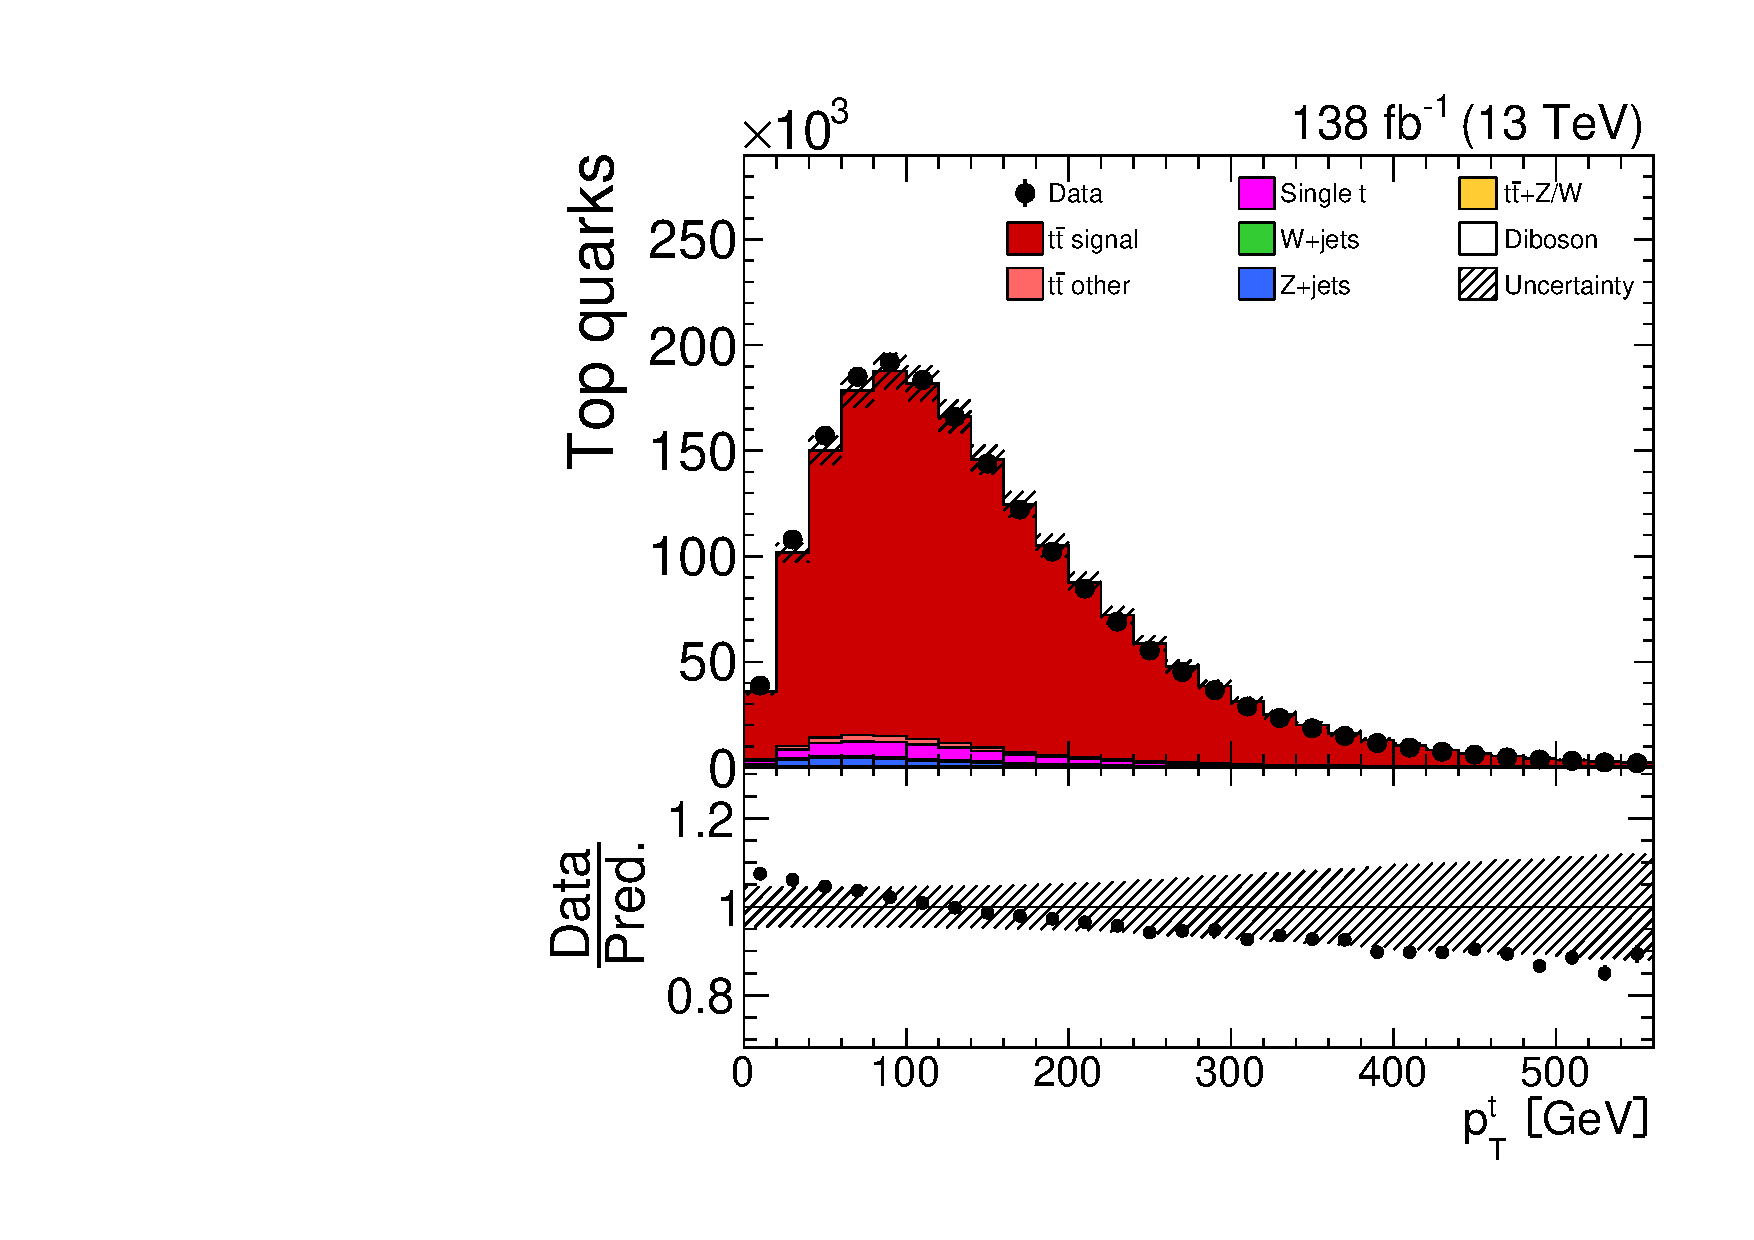
\includegraphics[width=0.30\textwidth]{fig_fullRun2UL/controlplots/combined/HypToppT.pdf}
%        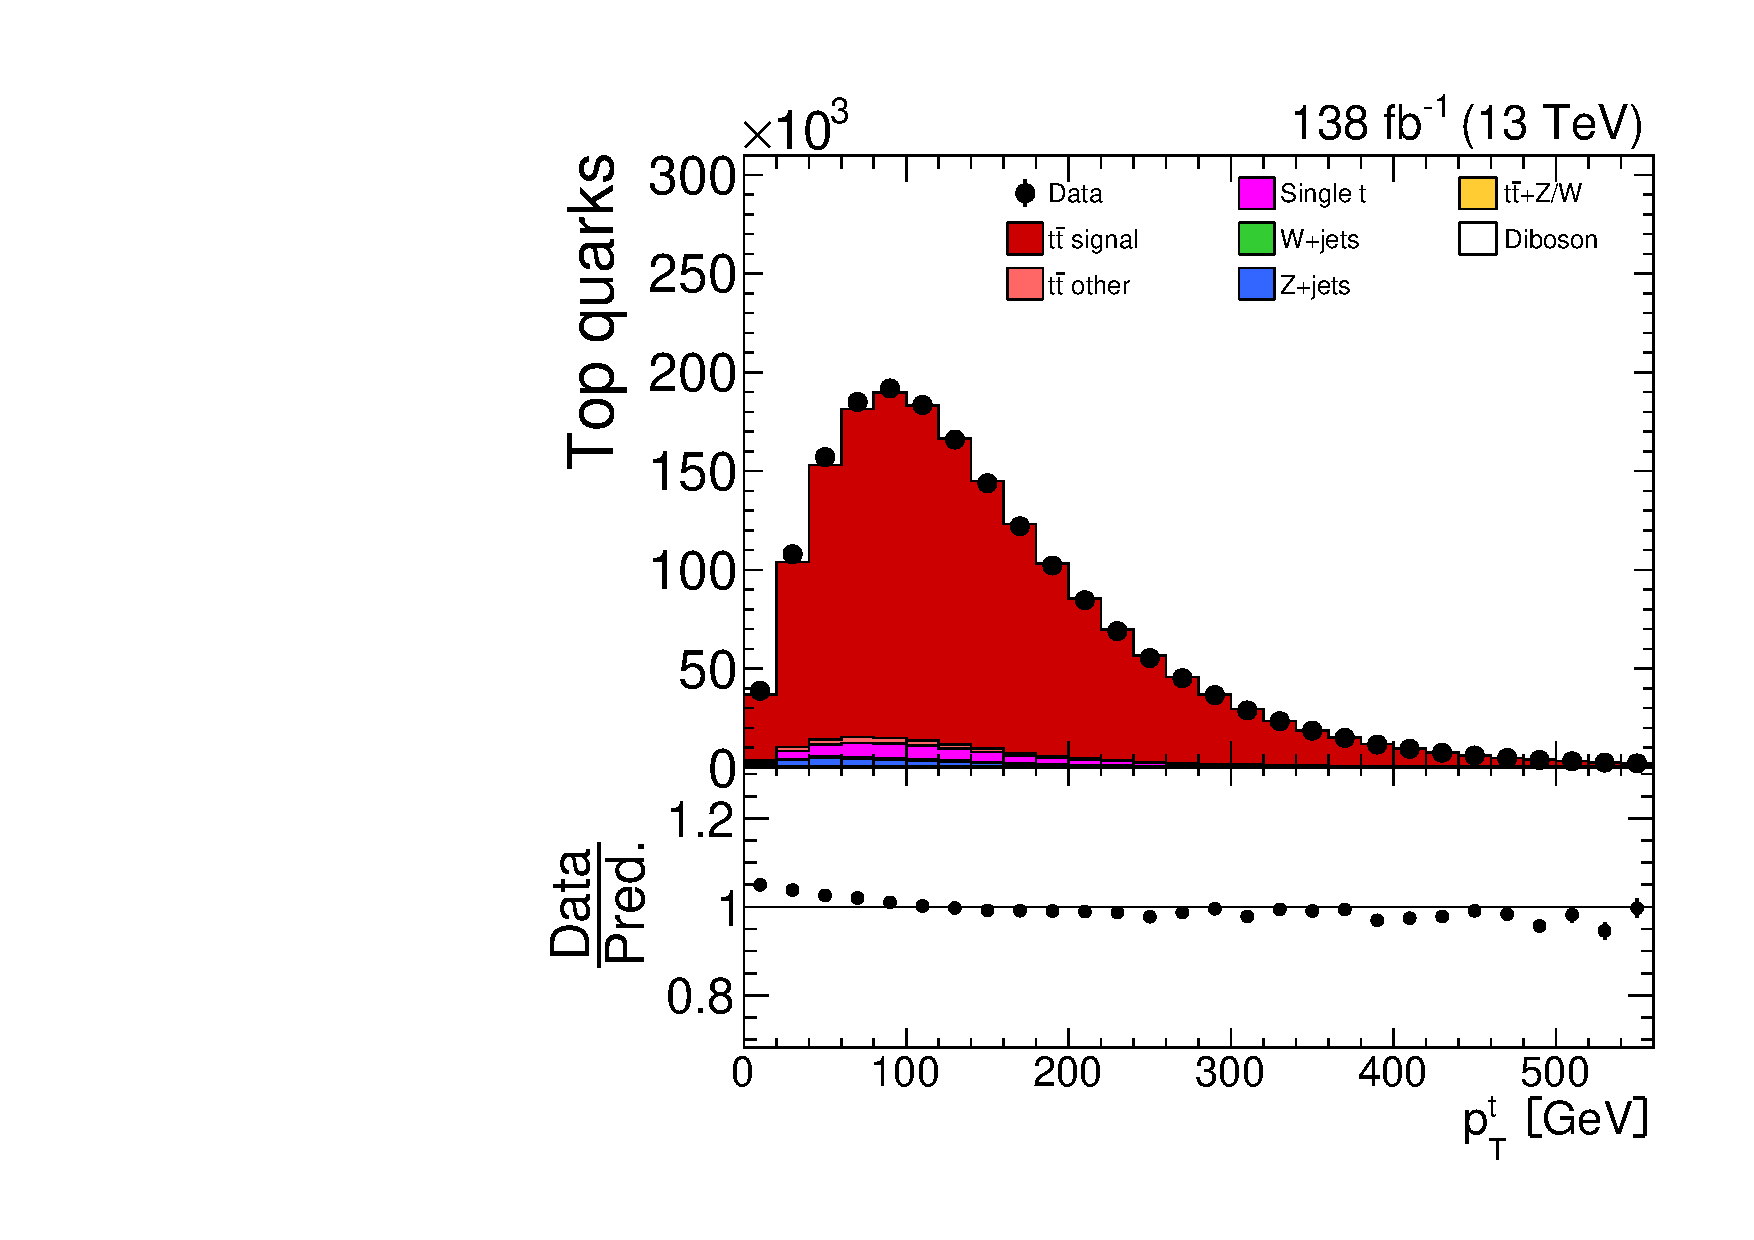
\includegraphics[width=0.30\textwidth]{fig_fullRun2UL/TOP_PT/combined/HypToppT.pdf}
      \end{center}
      \caption{\small Distribution of top \pT for Full Run II in the combined channel before (left) and after (right) top \pT reweighting.}      
      \label{fig:fullRun2ULtopptreweighting}
    \end{figure}
\end{itemize}
















